\documentclass{standalone}
\usepackage{tikz}
\usetikzlibrary{matrix,chains,positioning,decorations.pathreplacing,arrows}

\begin{document}
\tikzstyle{every node}=[font=\huge]

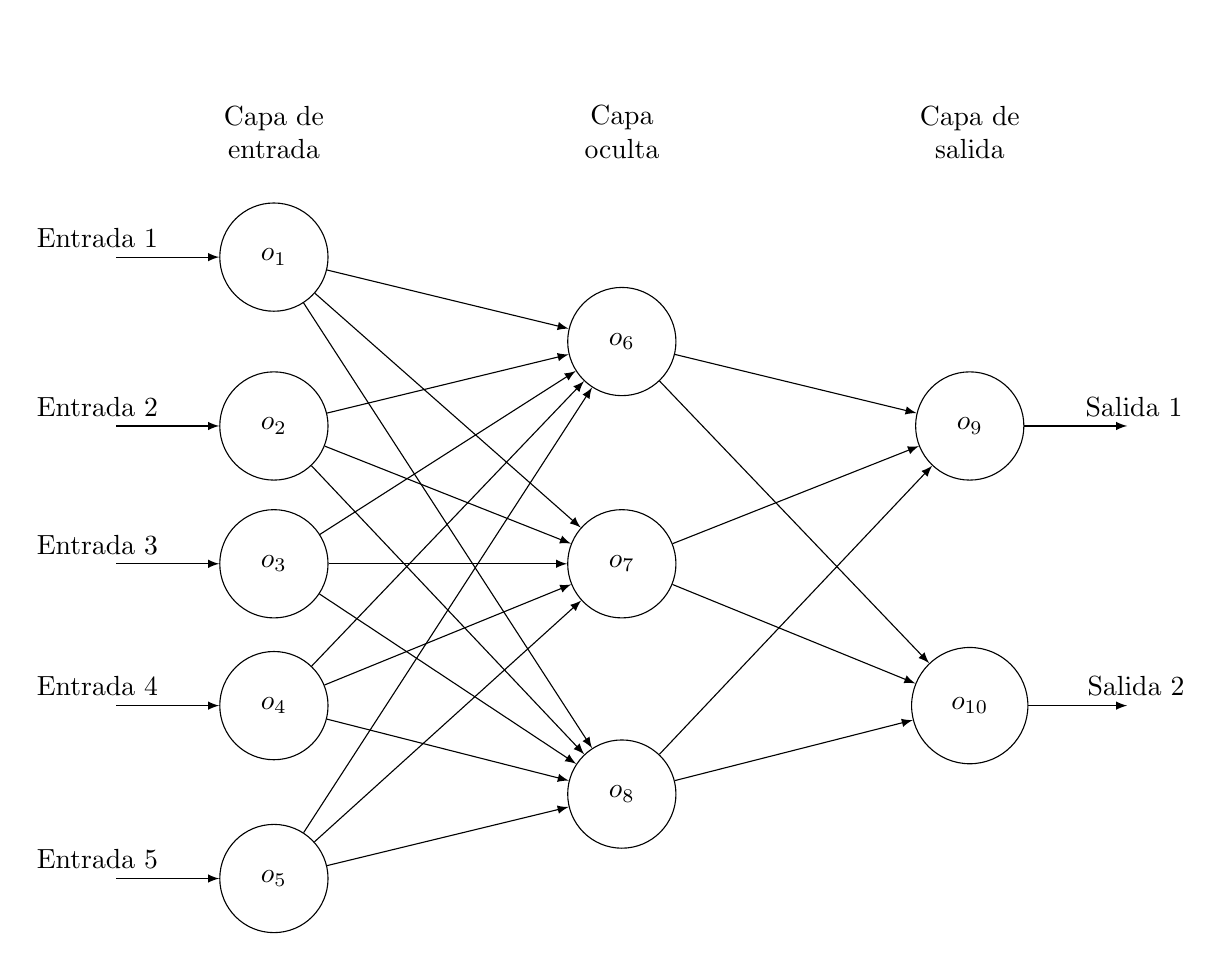
\begin{tikzpicture}[
plain/.style={
  draw=none,
  fill=none,
  },
net/.style={
  matrix of nodes,
  nodes={
    draw,
    circle,
    inner sep=10pt
    },
  nodes in empty cells,
  column sep=2cm,
  row sep=-9pt
  },
>=latex
]
\matrix[net] (mat)
{
|[plain]| \parbox{1.3cm}{\centering Capa de\\ entrada} & |[plain]| \parbox{1.3cm}{\centering Capa\\oculta} & |[plain]| \parbox{1.3cm}{\centering Capa de\\salida} \\
$o_1$ & |[plain]| \\
|[plain]| & $o_6$ \\
$o_2$ & |[plain]| & $o_9$\\
|[plain]| & |[plain]| \\
$o_3$ & $o_7$\\
|[plain]| & |[plain]| \\
$o_4$ & |[plain]| & $o_{10}$ \\
|[plain]| & $o_8$ \\
$o_5$ & |[plain]| \\
};
\foreach \ai [count=\mi ]in {2,4,...,10}
  \draw[<-] (mat-\ai-1) -- node[above left] {Entrada \mi} +(-2cm,0);
\foreach \ai in {2,4,...,10}
{\foreach \aii in {3,6,9}
  \draw[->] (mat-\ai-1) -- (mat-\aii-2);
}
\foreach \ai in {3,6,9}
{  
  \foreach \aii in {4,8}
    \draw[->] (mat-\ai-2) -- (mat-\aii-3);
}
   
\draw[->] (mat-4-3) -- node[above right] {Salida 1} +(2cm,0);
\draw[->] (mat-8-3) -- node[above right] {Salida 2} +(2cm,0);
\end{tikzpicture}


\end{document}